\documentclass[10pt,titlepage]{article}
\usepackage{fullpage}
\usepackage{listings}
\usepackage{graphicx}

\begin{document}
  \title{Lab4: iRobot Navigation in C}
  \author{Sam Mansfield and Toan Vuong\\
          TA: Hoekun Kim\\ 
          EECS149}
  \date{October 2nd, 2013}
  \maketitle

  \section{Introduction}

  \section{Analysis}
    %Analysis of algorithm used
     
    %State Machine 
      We ended up adding two new states, BACK and TURNRIGHT. When the iRobot is unpaused and senses an obstacle or cliff in the DRIVE state, it goes into obstacle avoidance mode and goes into the BACK state. The BACK state travels 50 mm backwards and goes into the TURNRIGHT state and the TURNRIGHT state, after making a right turn goes back into the DRIVE state. Figure 1 displays our final FSM.

      At the beginning of the lab we tried to create a more elaborate FSM and realized that we were actually making things more complicated to debug and therefore implement. By simplifying our design we created a better FSM. If I had to change one thing I would take out the square pattern, it makes the program more complicated to think about since you only have to correct within your square, which is a little odd considering that you will eventually be going in the corrected orientation after an obstacle eventually.
    
    \begin{figure}[h!]
      \centering
        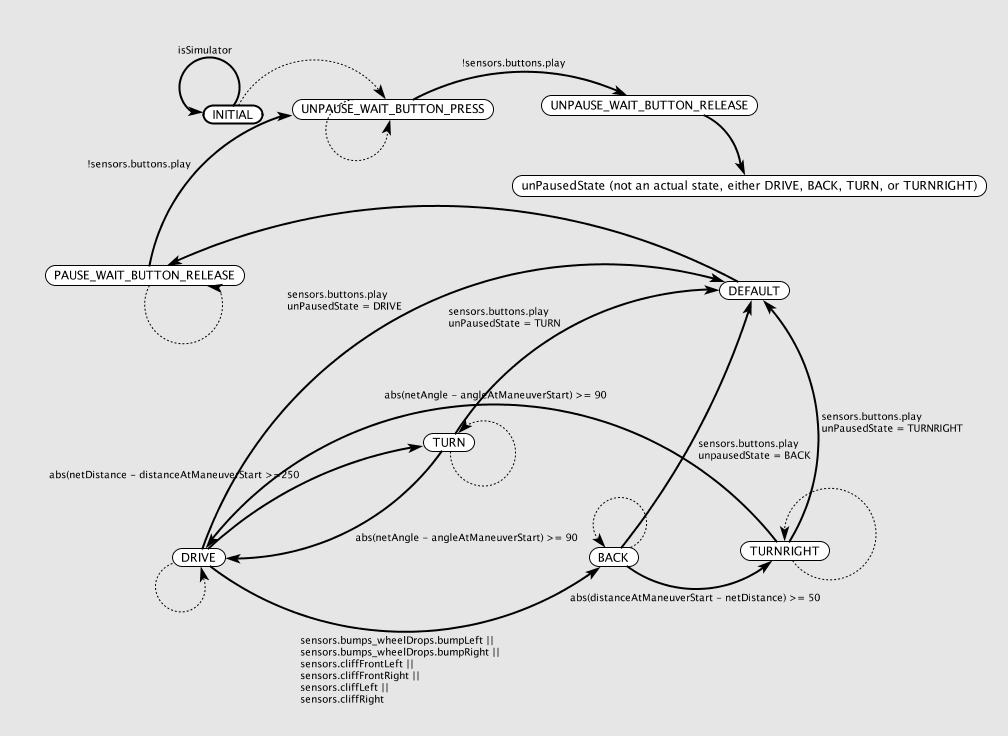
\includegraphics[width=1\textwidth]{../lab4_data/FSMLab4}
      \caption{Obstacle/Cliff avoidance FSM implemented in Lab 4}
    \end{figure}

  \section{Conclusion}
    Designing an obstacle/cliff avoidance algorithm was quite fun and rewarding when it actually worked. This was a very applicable problem for state machines and we can apply this technique to future problems that are similar in nature. This lab also helped us think about solving very simple human problems (avoiding an obstacle) step by step so that it can be applied to a robot.
\end{document}
